\documentclass{article}

\usepackage{tabularx}
\newcolumntype{L}[1]{>{\raggedright\arraybackslash}p{#1}} % linksbündig mit Breitenangabe
\newcolumntype{C}[1]{>{\centering\arraybackslash}p{#1}} % zentriert mit Breitenangabe
\newcolumntype{R}[1]{>{\raggedleft\arraybackslash}p{#1}} % rechtsbündig mit Breitenangabe

\usepackage{graphicx}
\usepackage{amsmath,amssymb,amsfonts,amsthm,mathtools} % Mathematik
\usepackage{subfigure} 
\usepackage{color}

\usepackage{pdfpages}

\usepackage[top=1.5cm, bottom=1.5cm]{geometry}

\usepackage{caption}

\title{Sheet 4 - Answers}
\author{Timm \& Boris}

\begin{document}
\maketitle

\section*{Task: 1}
Plot for the integrand of a two-dimensional Down-Out Call option with barrier B.
\begin{figure}[htbp]
  \centering
     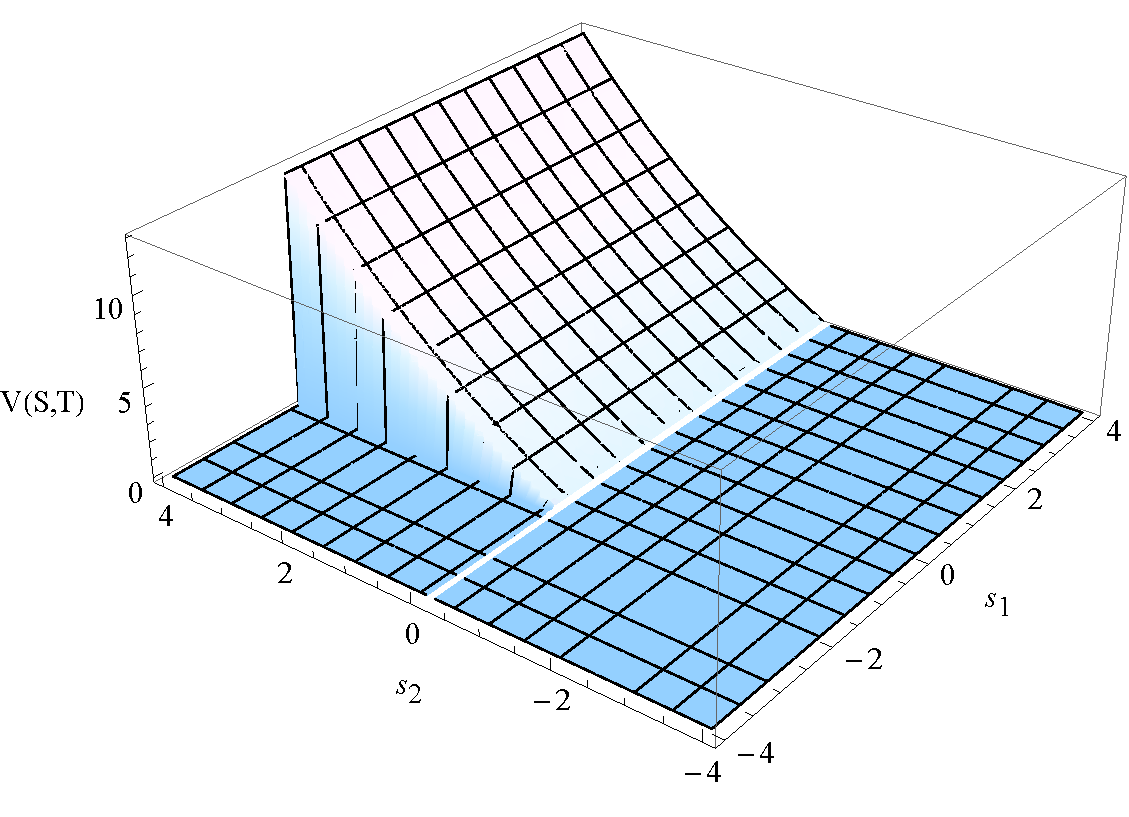
\includegraphics[width=1.0\textwidth]{../Task01/task01_plot.pdf}
  \caption*{Integrand of 2-dimensional Down-Out Call option.}
\end{figure}

\section*{Task: 2}
We get wrong values for our Monte Carlo and Quasi Monte Carlo method. We implemented this task (you can check the Code) but, we get false results.

\section*{Task: 3}
Plot of the Black Scholes formula for a Down-Out call option.
\begin{figure}[htbp]
  \centering
     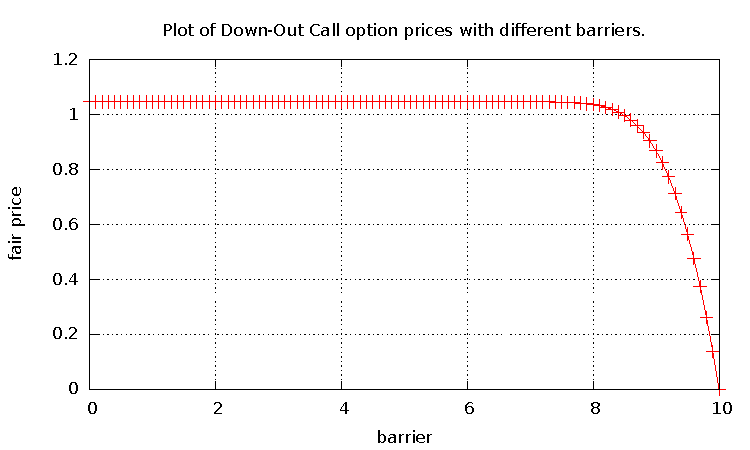
\includegraphics[width=1.0\textwidth]{../Task03/sh4_task3_price_plot.pdf}
%    \caption{}
\end{figure}


\newpage

\section*{Task: 4}
Monte Carlo convergence plots for different M.
% \begin{figure}[htbp]
%   \centering
%      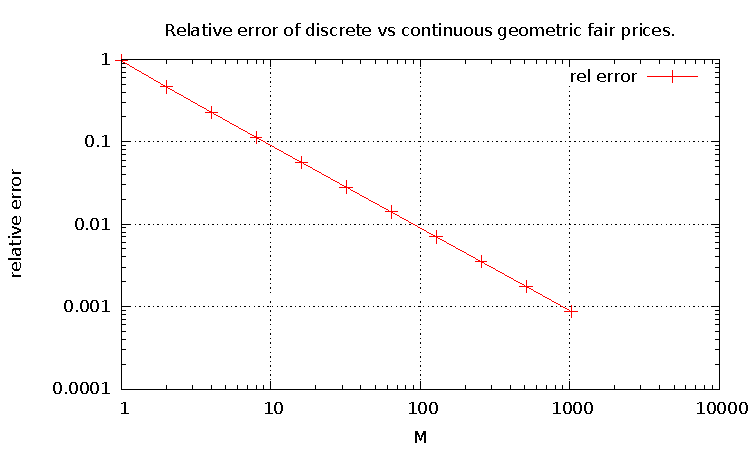
\includegraphics[width=1.0\textwidth]{../Task04/sh3_task4_convergence_plot.pdf}
% %    \caption{}
% \end{figure}

\section*{Task: 5}
Plot of the discrete time integrand for M = 2 with the usual parameters.
\begin{figure}[htbp]
  \centering
     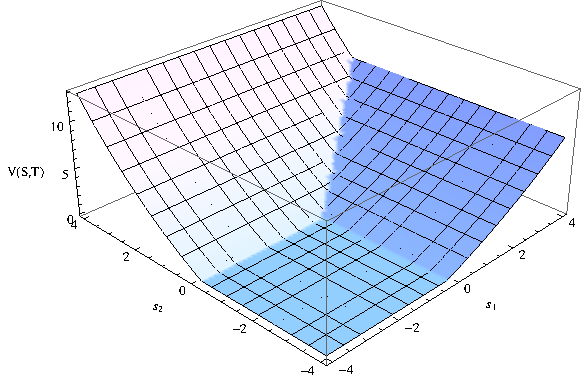
\includegraphics[width=0.8\textwidth]{../Task05/task05_plot.pdf}
%    \caption{}
\end{figure}

% \newpage
\section*{Task: 6}
Same as in Task 2. We implemented the Code and get a wrong convergence. You can look up the results in the Folder Task06 in the Sheet4 directory.

\section*{Task: 7}
Newton-Raphson algorithm with different start values $\sigma_0$ and for different actual $\sigma$ ($2 V / (\sqrt{T} S(0)) = 0.0975412$) for computing the implied volatility:
\begin{table}[htbp]%[tphp]
  \centering
  \renewcommand{\arraystretch}{1}
  \renewcommand{\tabcolsep}{0.25em} 
%   \scalebox{1.0}{
%   \ttfamily
  \begin{tabular}{p{2.0cm}|| R{1.6cm} |R{1.6cm} |R{1.6cm} |R{1.6cm} |R{1.6cm} }
%     \rowstyle{\bfseries}

actual $\sigma$ \textbackslash $\sigma_0$  & 0.0975412 & 0.0100000 & 1.0000000 &10.0000000 & 0.1000000\\
           \hline
           \hline
 0.0010000 & 0.0091670 & 0.0091670 &       nan &       nan & 0.0091670 \\
 0.0100000 & 0.0100000 & 0.0100000 &       nan &       nan & 0.0100000 \\
 1.0000000 & 1.0000000 &       nan & 1.0000000 &       nan & 1.0000000 \\
 9.0000000 & 9.0000000 &       nan & 9.0000000 & 9.0000000 & 9.0000000 

  \end{tabular}}
%   \large
%   \caption*{}

\end{table}

Put option prices computed with Newton-Raphson algorithm with different start values $\sigma_0$ and for different actual $\sigma$ ($2 V / (\sqrt{T} S(0)) = 0$): 
\begin{table}[htbp]%[tphp]
  \centering
  \renewcommand{\arraystretch}{1}
  \renewcommand{\tabcolsep}{0.25em} 
%   \scalebox{1.0}{
%   \ttfamily
  \begin{tabular}{p{2.0cm}|| R{1.6cm} |R{1.6cm} |R{1.6cm} |R{1.6cm} |R{1.6cm} }
%     \rowstyle{\bfseries}

actual $\sigma$ \textbackslash $\sigma_0$ & 0.0000000 & 0.0100000 & 1.0000000 &10.0000000 & 0.1000000\\
           \hline
           \hline
 0.0010000 & 0.0091670 & 0.0091670 &       nan &       nan & 0.0091670 \\
 0.0100000 & 0.0100000 & 0.0100000 &       nan &       nan & 0.0100000 \\
 1.0000000 & 1.0000000 &       nan & 1.0000000 &       nan & 1.0000000 \\
 9.0000000 & 9.0000000 &       nan & 9.0000000 & 9.0000000 & 9.0000000 
  \end{tabular}}
%   \large
%   \caption*{}

\end{table}

One observed cause for the divergence of the algorithm is that the quotient $\sigma_0 / \sigma$ diverges too far from one (either is too large or too near to zero).

\section*{Task: 8}

\section*{Task: 9}
We looked up some values from "{}www.onvista.de"{} and made screenshots of the entries we used. We used values of a Gold stock from UBS with same time of maturity and for European options.
\begin{figure}[htbp]
  \centering
     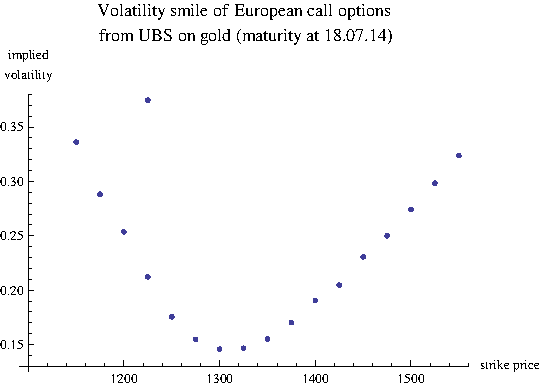
\includegraphics[width=1.0\textwidth]{../Task09/smileFromExternalData.pdf}
%    \caption{}
\end{figure}


\end{document}